\documentclass[lang=en,color=green]{elegantbook}
\title{Pragmatic Node.js development}
\subtitle{Primer in Nest.js}

\author{Zlatibor Zed Veljkovic}
\date{June 5, 2022}
\version{0.5}
\bioinfo{Email}{zveljkovic@hotmail.com}

\extrainfo{I had more time so it is short}

\setcounter{tocdepth}{3}


\logo{cule.jpg}
\cover{cover.jpg}

\definecolor{codebg}{rgb}{0.8,0.8,0.8}

% 本文档命令
\usepackage{array}
\usepackage{enumitem}
\usepackage[outputdir=./auxil]{minted}
\usepackage{mdframed}
\usepackage{hyperref}
\usepackage{graphicx}
\usepackage{color}


\newcommand{\ccr}[1]{\makecell{{\color{#1}\rule{1cm}{1cm}}}}
\newcommand{\ci}{\mintinline{bat}}
\newcommand{\bi}[1]{\textit{\textbf{#1}}}
\setmintedinline{bgcolor=codebg}
\AtBeginEnvironment{minted}{%
    \renewcommand{\fcolorbox}[4][]{#4}}

% 修改标题页的橙色带
% \definecolor{customcolor}{RGB}{32,178,170}
% \colorlet{coverlinecolor}{customcolor}
\begin{document}
    \maketitle
    \frontmatter

    \tableofcontents

    \mainmatter


    \chapter{Developer tools}\label{ch:developer-tools}
    Since ancient times, mankind has constantly spent effort to create new or to improve existing tools.
Even now, after thousands and thousands of years we are doing the same.
We are making new tools that will make us more efficient or at least to do our tasks easier.
In software development there are so many tools available it is hard to choose which set should be used.
Next sections will give simple overview of most prominent tools for each section.


\section{Command line interfaces}\label{sec:command-line-interfaces}
Command line interfaces (CLI) are programs that use console/textual interface and allow you to interact with it.
Every operating system comes with one or more of these, Windows has Command Prompt (aka cmd.exe) and PowerShell,
Linux has sh and bash with many alternatives (commonly known as shell), and macOS has Terminal.app.
One issue that novice developers struggle is that when someone tells you to “open the terminal”,
they mean one for your system.

Before mentioned apps are the ones that allow you to execute some commands or run different programs.
There are also some CLI that is specifically built for one purpose.
One example would be Nest.js CLI which allows you to quickly create new projects,
update dependencies or start the Nest app.

\subsection{Command prompt}\label{subsec:command-prompt}
Command prompt comes preinstalled on Windows systems.
It supports batch scripts and usually the file is with .bat extension.

\noindent\begin{minipage}[t]{0.5\textwidth}%
    \centering{Pros}
    \begin{itemize}[leftmargin=*]
        \item Available on all Windows systems
        \item Allows executing programs in current directory without  \lstinline{.\}  prefix
    \end{itemize}
\end{minipage}%
\begin{minipage}[t]{0.5\textwidth}%
    \centering{Cons}
    \begin{itemize}[leftmargin=*]
        \item Batch scripting language is really outdated and hard to write more complex stuff
        \item No command history search
    \end{itemize}
\end{minipage}%

\begin{figure}[htbp]
    \centering
    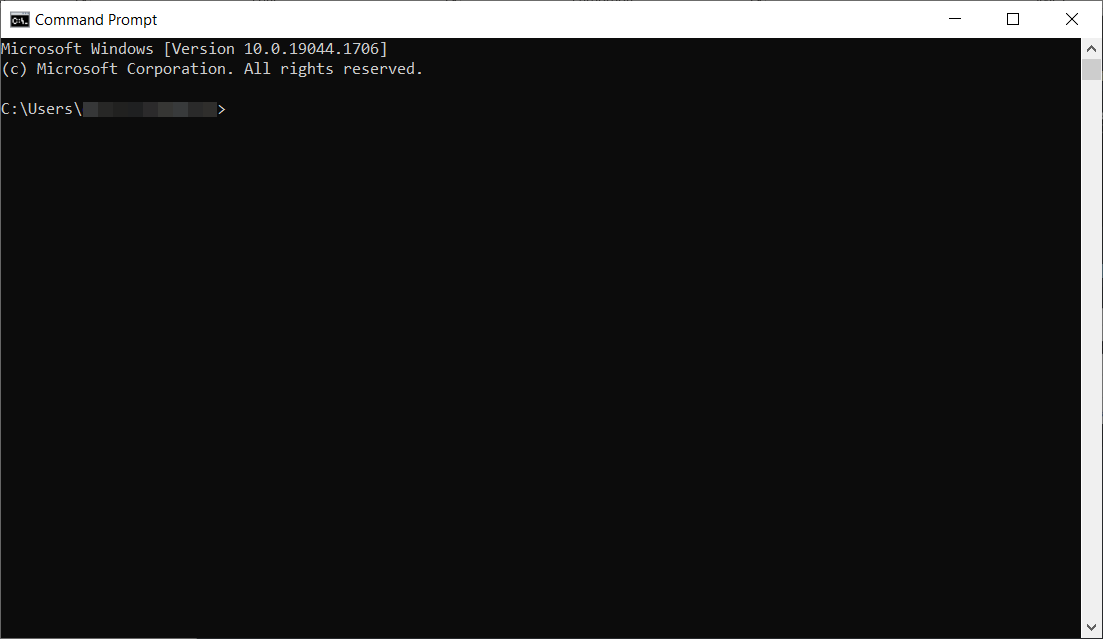
\includegraphics[width=0.6\textwidth]{images/command-prompt}
    \caption{Command Prompt\label{fig:Command Prompt}}
\end{figure}

Reference for available Command Prompt commands can be found at \href{https://docs.microsoft.com/en-us/windows-server/administration/windows-commands/windows-commands}{Windows Commands}

\subsection{PowerShell}\label{subsec:powershell}
Another shell for Windows systems is called PowerShell, and it is available from Windows 7 or later operating systems.
Open source version PowerShell Core was released in 2016, and it is based on .Net Core which also made it cross-platform.
It has better integration with various functionalities available in Windows so it is prefreed choice over Command Prompt
when working with system administration.
For developer work it might be an overkill.


\noindent\begin{minipage}[t]{0.5\textwidth}%
    \centering{Pros}
    \begin{itemize}[leftmargin=*]
        \item Available on all Windows systems
        \item Better integration with Windows functionalities
        \item Has command history search (with F8 key)
    \end{itemize}
\end{minipage}%
\begin{minipage}[t]{0.5\textwidth}%
    \centering{Cons}
    \begin{itemize}[leftmargin=*]
        \item  Does not allow executing programs in
              current directory without  \lstinline{.\} prefix
    \end{itemize}
\end{minipage}%

\begin{figure}[htbp]
    \centering
    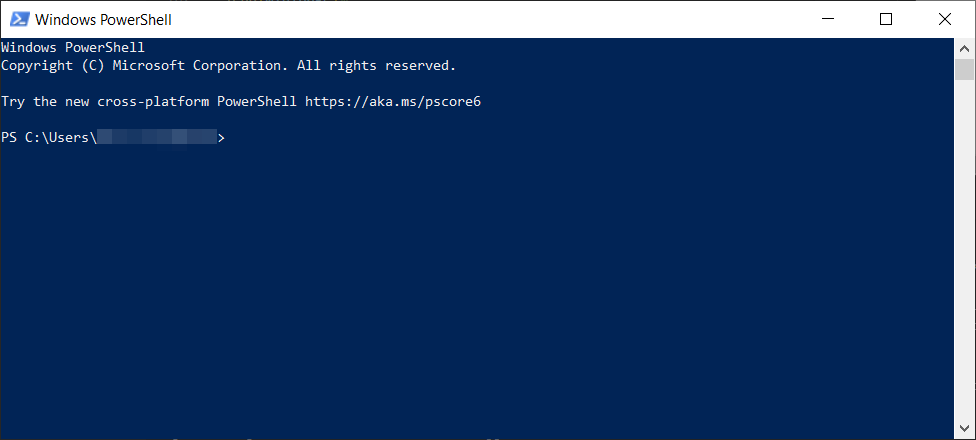
\includegraphics[width=0.6\textwidth]{images/powershell}
    \caption{PowerShell\label{fig:PowerShell}}
\end{figure}

\subsection{Linux/Mac terminals/shells}\label{subsec:linux/mac-terminals/shells}

Linux and Mac have much bigger choice of terminals.
Terminal refers to a program that allows you to run
programs which are known as shells. Shells come in lots of varieties sh, bash, ksh, csh, zsh\dots.
Linux has many command line programs that allow you to manipulate output of commands and
offers a lot for power users.


\section{Package managers}

Package managers can be used to install additional software on your PC. They usully automate process of
downloading, installing and configuring software. Later it also helps with keeping the installed software
up to date or with removal.

\begin{itemize}[leftmargin=*]
    \item Chocolatey is most prominent Windows package manager. It can be downloaded from \href{https://chocolatey.org/}{https://chocolatey.org/}.
          Searching for packages is done with \mintinline{bat}{choco search postgresql}
          and installation with \mintinline{bat}{choco install postgresql} will install Postgres.
    \item Homebrew is a Mac OS X package manager written in Ruby.
          It can be downloaded from \href{https://brew.sh}{https://brew.sh}.
          Command \mintinline{bat}{brew search postgres}
          is used to search for package while \mintinline{bat}{brew install postgresql} to install a package.
    \item Linux has many package managers and preferred way is to use package manager
          that comes with operating system.
\end{itemize}

    \chapter{NestJS application recommendations}\label{ch:nestjs-application-recommendations}
        \section{NestJS}\label{sec:nestjs}

    I couldn't explain it better than the words of the author ``Nest (NestJS) is a framework for building
    efficient, scalable Node.js server-side applications.
    It uses progressive JavaScript, is built with and fully supports
    TypeScript (yet still enables developers to code in pure JavaScript)
    and combines elements of OOP (Object-Oriented Programming),
    FP (Functional Programming), and FRP (Functional Reactive Programming).''

    The documentation is found on \href{https://docs.nestjs.com/} where you can
    read all about framework components.
    Some components are not up to task and in further sections we will focus on good and bad
    sides of available components and some alternatives.


    \section{Environments}\label{sec:environments}
    Modern apps usually run in multiple environments.
    My recommendation for environments is with code name in parenthesis.

    \begin{itemize}
        \item Local development environment (\bi{a})
        \item Local testing environment (\bi{b})
        \item Public development environment (\bi{d})
        \item Public stable development environment (\bi{s})
        \item CI testing environment (\bi{t})
        \item Public quality assurance environment (\bi{q})
        \item Public production environment (\bi{p})
    \end{itemize}

    \subsection{Local development environment}\label{subsec:local-development-environment}
    Local development environment is pretty obvious as each developer
    is running the application on development machine.
    Code name to be used for this environment is \bi{a} which as a letter
    represents first letter in alphabet so this environment represents
    first step in the application development.

    \subsection{Local testing environment}\label{subsec:local-testing-environment}
    Local testing environment (\bi{b}) is where developer runs tests on development
    machine.
    This environment is necessary to isolate testing of the app
    completely from local development environment.
    Without this isolation
    data that has been entered during development could influence
    test running.
    We usually use same variables as \bi{a} env, but we usually want to change external dependencies
    like database/queues/Kafka/storage so test runs are properly isolated.

    \subsection{Public development environment}\label{subsec:public-development-environment}
    Public development environment is the environment which contains the
    latest application code.
    It is configured to be automatically built
    from the \bi{develop} branch.
    This environment is meant to be
    broken/reset at any time.
    It is also first public environment for use
    mostly by developers.

    \subsection{Public stable development environment}\label{subsec:public-stable-development-environment}
    Public stable development environment \bi{s} is the environment that is
    manually updated.
    When team is happy with the state of \bi{d} environment
    they can promote it to this environment.
    This allows team leads
    to test the app without interruptions that would come if they used \bi{d}
    environment.

    \subsection{CI testing environment}\label{subsec:ci-testing-environment}
    CI testing environment is used during the PR verifications in the build
    pipelines.
    This is necessary for same reasons as local testing environment,
    just on the public side.

    \subsection{Public quality assurance environment}\label{subsec:public-quality-assurance-environment}
    Public quality assurance environment \bi{q} is environment meant
    for external evaluation.
    When all issues identified in \bi{s} environment
    are fixed and team lead is happy with its state, this build can be promoted
    to \bi{q} environment.
    This environment should be same in specs as
    public production environment, so it can be also used as database
    migration verification or as performance test target.

    \subsection{Public production environment}\label{subsec:public-production-environment}
    Public production environment \bi{p} is environment that is available to the
    users of the application.
    This makes it last step in build - release cycle.
    As real users are using it this environment should be under constant monitoring.


    \section{Environment zones}\label{sec:environment-zones}
    All of the environments can be grouped in production and non-production zones.
    The app code can then provide developers with:
    \begin{itemize}
        \item More information about errors for example by outputting
        stack traces, displaying error data, and various other info which should be
        hidden from the real users.
        \item Improve testability by including features to log in as certain type
        of users, commands that will precreate certain data sets, etc\dots
        \item Distinguish between seeding production data and developer data.
    \end{itemize}


    \section{Application Configuration}\label{sec:application-configuration}

    Application configuration in modern development is inescapable.
    NestJS
    offers a component \bi{ConfigService} which is using \bi{dotenv} package internally.
    What we get is a way to load .env environment file and access the variables
    defined in environment.

    What we are missing is:
    \begin{itemize}
        \item Checking that all required variables are supplied
        \item That variables conform to the expected type (configuration schema)
        \item Ability to use multiple .env files so that you can easily configure
        local development environment (\bi{a}) and local testing environment (\bi{b})
        for example by having \bi{.env.b} file overriding database name from \bi{.env}
        used by local development environment.
        \item Type safety as we need to use string identifiers when getting the
        values
    \end{itemize}

    Package \href{https://www.npmjs.com/package/convict}{convict} has almost all
    of the above but has a requirement that each setting has default value
    which will not fail the startup if required variable is not found in
    environment variables.

    \subsection{Zeddy Config}\label{subsec:zeddy-config}
    Zeddy Config is my \href{https://www.npmjs.com/package/zeddy-config}{library}
    heavily inspired by \href{https://www.npmjs.com/package/convict}{convict} but offers
    type safety without default values and is offering just enough functionality
    for any app.
    This package also provides variable loading from the \bi{.env}
    and \bi{.env.env-name} files with the \bi{dotenvize} method.
    With this simple
    packages we cover all missing elements for good config:
    \begin{itemize}
        \item Single method load the environment variables into JS variable.
        \item Validation of the configuration schema.
        \item Full type safety as schema type property is transferred to config object properties.
        \item It also has additional method to load multiple .env files (\bi{dotenvize}).
    \end{itemize}

    \begin{minted}{javascript}
import { configz, dotenvize } from "zeddy-config";

dotenvize();

export const config = configz({
  env: {
    description: "Running environment",
    envVar: "NODE_ENV",
    type: "string"
  },
  server: {
    description: "Server info",
    type: "object",
    properties: {
      port: {
        description: "Server port",
        envVar: "SERVER_PORT",
        type: "int",
        validator: (port) => {
          return port === 3000;
        }
      },
      host: {
        description: "Server host",
        envVar: "SERVER_HOST",
        type: "string"
      },
    }
  }
});

// resulting config interface is {env: string; server: {port: number; host: string}}
}
    \end{minted}


    \section{Exceptions and errors}\label{sec:exceptions-and-errors}

    Usually people use one or the other term to represent both errors and exceptions
    but these terms, while both having the same root of something unexpected occurred,
    have a difference that exceptions can be handled, while error shouldn't be handled.

    For example, if we try to open a file which does not exist we should get an
    FileNotFoundException exception.
    Normal application will handle that exception to
    inform the user about missing file and continue working normally.

    Errors on the other way prevent the program from running or even compiling.
    One of the frequent errors is SyntaxError which happens when we don't follow
    language constructs such as using undeclared variable or misspelling the keywords.
    This type of error is also called compile time error as it is thrown
    when compiling the application.
    Other type of errors are runtime errors
    which happen during the application run.
    Usually these errors would lead to
    app ending or restarting.
    For example if we do not have enough memory on
    the system we will get OutOfMemoryError, and best the app can do is to end/restart.

    \subsection{REST Api Errors/Exceptions and HTTP Status Codes}
    \label{subsec:rest-api-errors/exceptions-and-http-status-codes}

    HTTP Status Codes are defined in \href{https://httpwg.org/specs/rfc9110.html#overview.of.status.codes}{RFC 9110}
    which groups the statuses codes (100-599) in five categories:
    \begin{itemize}
        \item 100--199 are informational codes (101 Switching Protocols)
        \item 200--299 are success codes (200 OK)
        \item 300--399 are redirect codes (301 Moved Permanently)
        \item 400--499 are client error code (404 Not Found)
        \item 500--599 are server error code (500 Internal Server Error)
    \end{itemize}

    REST APIs are able to return the result of the action or error/exception
    and most frameworks like NestJS are tying the errors with server codes.
    One example would be if we search the database by id and don't find the
    object we can throw NestJS NotFoundException which will use 404 http status code.

    \subsection{Recommendations for HTTP call errors}\label{subsec:recommendations-for-http-call-errors}

    My recommendation is to use only two HTTP Status Codes:
    \begin{itemize}
        \item 400 for all exceptions where client retries would not change the outcome.
        This should represent that user has sent wrong data or not allowed to do something.
        If something doesn't change this request would never succeed.
        \item 500 for all errors where client retries could succeed after some timeout.
        This might be thrown when cache is refreshing, or there is loss of network connectivity
        to some other services.
    \end{itemize}

    When exception is being returned to the HTTP client, in addition to HTTP Status Code,
    we also need to return more data about the error in response body.
    These response bodies should be more or less detailed depending on the environment zone the app is running.
    In \bi{prod zone} we should output only exception id and generic name of the error,
    while in \bi{dev zone} we can additionally send more data or stack trace.

    Also, JavaScript and NestJS error implementation provide short description of the exception/error,
    with \bi{message} property - which is not recommended.
    Having many exceptions/errors with unique name is better for responding and providing proper error description with
    the translation tooling.
    Having errors translated on the client (frontend) is much preferable as the clients/frontends are translated more often than backends.
    We have frequently seen
    multilingual content on websites but rarely (if ever) translated versions of endpoint URLs or
    POST data names.
    Additional point is that if we have multiple clients (web and mobile app)
    each of those can define their own user presentation of that error which is not possible
    with fixed description returning from backend.

    Fine-grained exception/errors are preferred and naming should reflect those, and build
    from something larger to something smaller.
    For example \bi{AuthorizationTokenBearerMissingException},
    \bi{AuthorizationTokenExpiredException}, \ldots If possible we should group certain exceptions into
    one by providing additional parameters as we have entity field in \bi{EntityNotFoundException(\{entity: User, id: '1234'\})}
    and \bi{EntityNotFoundException(\{entity: UserProfile, id: '1234'\})}.

    Exceptions/errors should be easy to make, and they should be grouped together with relevant
    errors instead of all in one place or each for it self.

    \subsection{Zeddy Errors}\label{subsec:zeddy-errors}

    Zeddy Errors is npm package \href{https://www.npmjs.com/package/zeddy-errors}{https://www.npmjs.com/package/zeddy-errors} that follows recommendations 
    from \hyperref[sec:REST Api Errors/Exceptions and HTTP Status Codes]{REST Api Errors/Exceptions and HTTP Status Codes}.
    It features most simple creation of new errors, allows groups of errors, ease of import,
    type safety and ease of use.
    It has 0 dependencies except TypeScript and integrates well into
    any existing frameworks.
    There is a sample NestJS project available at \href{https://github.com/zveljkovic/zeddy-errors-example}(https://github.com/zveljkovic/zeddy-errors-example).

    Usage is simple, export error group with defined errors with optional generic argument about the data type,
    import it where needed and throw the new instance.

    \begin{minted}{javascript}
// file: shared.errors.ts
export const SharedErrors = {
  EntityNotFound: class extends ExceptionBase<{ type: string; id: number }> {},
  JwtTokenMissingBearer: class extends ExceptionBase{},
  IntentionalError: class extends ErrorBase<{ reason: string }> {},
};

// file: some.service.ts
import {SharedErrors} from './shared.errors';
//...
throw new SharedErrors.IntentionalError({reason: "Testing errors"});
throw new SharedErrors.JwtTokenMissingBearer();

    \end{minted}


    \section{Logging}\label{sec:logging}

    Logging is one of the most basic but very important aspect of application development.
    Logs provide the insight into application processing, helps you reproduce the bugs,
    and can be used as visible comments.

    Modern logging should be:
    \begin{itemize}
        \item Effortless.
        The easier the logs are to write the more developers will use them.
        \item Centrally configured.
        Logging configuration should live in one file, so it is easy to modify and extend.
        \item Optimized for different environments.
        For example on local environments we want
        logs to be in plain format printed to standard output, so developers can read them,
        but for remote environments logs can be in json format for shipping to ELK stack for example.
        \item Adaptable.
        Logger should be easy to adapt to specific services.
        For example
        integrating with Azure's App Insights.
        \item Versatile.
        It's not rare that logs need to be sent to multiple services.
        Sending
        logs to ELK stack for long-lasting storage and to Azure AppInsights is common practice.
    \end{itemize}

    Many of standard libraries

    \chapter{NestJS component guide}\label{ch:nestjs-component-guides}
    To better understand the available architectural guides in NestJS we need to shortly introduce ourselves with
core building blocks of NestJS\@.

\subsection{NestJS Modules}\label{subsec:nestjs-modules}

NestJS has is able to modularize the code with Module classes.
Each application must have at least one module but can have many modules.
These modules can contain multiple classes, and they have an interface with which we can specify
what is available from the modules importing it.
This allows us to have separation of concerns, by creating self-sufficient modules with public interfaces
(by specifying public classes in exports field of module).
For example, we can create UserModule that will provide UserService class to any module importing UserModule.
Parent modules will be able to get the UserService object via dependency injection system, but they couldn't
get the ``private'' classes used within module like UserRepository, UserEmailService, UserController and others unless
explicitly exported from the module.
This allows to hide internal implementation of the module and force usage of exported classes
to interact with this module.

\subsection{NestJS Providers}\label{subsec:nestjs-providers}
NestJS concept of provider is very large but can be sumarized as a class that can be injected through NestJS dependency
injection system.
Many of the NestJS basic classes are providers like services, repositories, helpers, controllers, etc\ldots
Class can be treated as a provider if it has @Injectable annotation and is defined in modules provider field.

\subsection{NestJS Controllers}\label{subsec:nestjs-controllers}

NestJS has built-in support for Controllers.
They are objects that define endpoints that allow the user to interact with the application.
For each endpoint controllers specify which URL, and HTTP method are required to trigger it.
Also, controllers serve as a place to define expected request parameters, validation, authorization, and most importantly
to trigger the specific code to handle that request.

\subsection{NestJS Middleware, Exception Filters, Pipes, Guards, Interceptors}\label{subsec:nestjs-others}
The rest of NestJS components are essentially a way to interact with request before it reaches controller.
Short explanation of each follow but for more in-depth explanation please read official documentation.

\begin{itemize}
  \item Middleware - code that runs before the routing.
  \item Exception filters - code that will allow you to react to unhandled exception from your code.
  \item Pipes - used for transformation and validation of data before execution of controller.
  \item Guards - checking if request is allowed to be executed by controller (authentication and authorization).
  \item Interceptors - wrap controller execution so you can write code that is executed before or after controller execution
\end{itemize}


    \chapter{NestJS architectural guides}\label{ch:nestjs-architectural-guides}
    Depending on the expected size and complexity, application architecture should be designed to maximise productivity,
and minimise complexity but without sacrificing the maintainability or development of possible future requirements.
There are various online topics on subject of architecture and their applicability, so we will shortly focus on most
common types of errors during architecture design.

Over-engineering: this happens when solution is unnecessarily complicated.
There are many examples of this but most common ones are:
\begin{itemize}
  \item designing for multiple databases in agnostic way when 99% of projects never switch the database type (i.e. going from Postgresql to Sql Server).
  \item using microservice architecture where hidden cost of included complexity on both developer and devops side is not
  properly compared to the benefits of this approach.
  \item designing for infinite customisation of the components.
\end{itemize}

Under-engineering (Hacky): this happens when solution is not using parts for intended purposes but is tried to repurpose
existing ones in different way (which often fails).
Some of these are:
\begin{itemize}
  \item using database instead of in memory cache.
  \item using self-made code for distributed task scheduling (please use ZooKeeper).
  \item using cron jobs instead of proper background task processing.
\end{itemize}


This section will focus on most commonly used architectural practices for building NestJS based backend applications
in increasing complexity.

\section{Arch: As Simple As It Gets}\label{sec:arch-as-simple-as-it-gets}

The most basic setup we can have is to have one module that has one controller defined.
All the code gets written in the controller method.
This is only suitable for quick POC maybe when testing new libraries and later thrown away.
But even then it is a questionable practice as it might be easier to test it in main project.

\section{Arch: One module project based with services based on db entities}\label{sec:arch-om-db}

One module project will have no modularization but can have multiple controllers, services and other NestJS components.
Modularization is emulated with the folder structure and this works really well for POC or small projects.
Mainly for smaller projects there is 1:1 correlation between controllers and services.
Downside of this approach is that availability of each app component may tempt usage of classes that should be private
if there was proper modularization.
One example would be to update user directly via UserRepository instead of going through the UserService as it requires
all attributes to be specified.
Later, for example if we wanted to send a confirmation email everytime user is updated we would have to find all places
where UserRepository was used and add code there.

\section{Arch: Multi module project with services based on db entities}\label{sec:arch-mm-db}

An expansion on previous architecture is that now we are using multiple modules properly
(by forbidding imports of classes that are not exported from modules), but we still have groupings around entities.
This way we have multiple modules, well-defined public interfaces but if application grows in complexity we may start
encountering cyclic dependencies.
Cyclic dependencies mostly happen in services, and reason is that two service require each other to do the job.
For simplistic example we can say that UserService and WorkService have a cyclic dependency
when WorkService needs UserService to fetch the user, while UserService in deleteUser method needs WorkService
to remove all the Work entities for current user.

\section{Arch: Multi module project with services based on Domain Driven Design}\label{sec:arch-mm-ddd}

To solve the previous issue we can try the DDD and model services around business domains, and that might help a bit,
but when domain interactions become more complex we might still experience the cyclic dependency issue.

\section{Arch: Multi module project with services based on Domain Driven Design plus events}\label{sec:arch-mm-ddd-events}

To fight cyclic dependencies arising from large service classes, and make them independent of other modules we might
start to utilize internal events.
By raising events we may handle some cases in parts of other modules.
For example, in UserService we can use exported class UserEvents to raise UserCreated event, and then the
EmailService can respond to that event without needing a DI link to UserService.
This will help greatly in decoupling the modules and making app more maintainable for larger projects.

\begin{tcolorbox}[title=Dependency Injection issues]
  It becomes obvious at this point that dependencies should be scoped to the point of the usage.
  Having large service classes that depend on the other big service classes, we will come to the point where we
  will have to fight with cyclic dependencies.
  But it's not only that, why do we need to instantiate a service if it is used in only one method.
  We need a new (old) approach.
\end{tcolorbox}




    \chapter{NestJS testing}\label{ch:nestjs-testing}
    To better understand the available architectural guides in NestJS we need to shortly introduce ourselves with
core building blocks of NestJS\@.

\subsection{NestJS Modules}\label{subsec:nestjs-modules}

NestJS has is able to modularize the code with Module classes.
Each application must have at least one module but can have many modules.
These modules can contain multiple classes, and they have an interface with which we can specify
what is available from the modules importing it.
This allows us to have separation of concerns, by creating self-sufficient modules with public interfaces
(by specifying public classes in exports field of module).
For example, we can create UserModule that will provide UserService class to any module importing UserModule.
Parent modules will be able to get the UserService object via dependency injection system, but they couldn't
get the ``private'' classes used within module like UserRepository, UserEmailService, UserController and others unless
explicitly exported from the module.
This allows to hide internal implementation of the module and force usage of exported classes
to interact with this module.

\subsection{NestJS Providers}\label{subsec:nestjs-providers}
NestJS concept of provider is very large but can be sumarized as a class that can be injected through NestJS dependency
injection system.
Many of the NestJS basic classes are providers like services, repositories, helpers, controllers, etc\ldots
Class can be treated as a provider if it has @Injectable annotation and is defined in modules provider field.

\subsection{NestJS Controllers}\label{subsec:nestjs-controllers}

NestJS has built-in support for Controllers.
They are objects that define endpoints that allow the user to interact with the application.
For each endpoint controllers specify which URL, and HTTP method are required to trigger it.
Also, controllers serve as a place to define expected request parameters, validation, authorization, and most importantly
to trigger the specific code to handle that request.

\subsection{NestJS Middleware, Exception Filters, Pipes, Guards, Interceptors}\label{subsec:nestjs-others}
The rest of NestJS components are essentially a way to interact with request before it reaches controller.
Short explanation of each follow but for more in-depth explanation please read official documentation.

\begin{itemize}
  \item Middleware - code that runs before the routing.
  \item Exception filters - code that will allow you to react to unhandled exception from your code.
  \item Pipes - used for transformation and validation of data before execution of controller.
  \item Guards - checking if request is allowed to be executed by controller (authentication and authorization).
  \item Interceptors - wrap controller execution so you can write code that is executed before or after controller execution
\end{itemize}


\end{document}
